% Options for packages loaded elsewhere
\PassOptionsToPackage{unicode}{hyperref}
\PassOptionsToPackage{hyphens}{url}
\PassOptionsToPackage{dvipsnames,svgnames,x11names}{xcolor}
%
\documentclass[
  11pt]{article}

\usepackage{amsmath,amssymb}
\usepackage{iftex}
\ifPDFTeX
  \usepackage[T1]{fontenc}
  \usepackage[utf8]{inputenc}
  \usepackage{textcomp} % provide euro and other symbols
\else % if luatex or xetex
  \usepackage{unicode-math}
  \defaultfontfeatures{Scale=MatchLowercase}
  \defaultfontfeatures[\rmfamily]{Ligatures=TeX,Scale=1}
\fi
\usepackage{lmodern}
\ifPDFTeX\else  
    % xetex/luatex font selection
\fi
% Use upquote if available, for straight quotes in verbatim environments
\IfFileExists{upquote.sty}{\usepackage{upquote}}{}
\IfFileExists{microtype.sty}{% use microtype if available
  \usepackage[]{microtype}
  \UseMicrotypeSet[protrusion]{basicmath} % disable protrusion for tt fonts
}{}
\usepackage{xcolor}
\setlength{\emergencystretch}{3em} % prevent overfull lines
\setcounter{secnumdepth}{5}
% Make \paragraph and \subparagraph free-standing
\makeatletter
\ifx\paragraph\undefined\else
  \let\oldparagraph\paragraph
  \renewcommand{\paragraph}{
    \@ifstar
      \xxxParagraphStar
      \xxxParagraphNoStar
  }
  \newcommand{\xxxParagraphStar}[1]{\oldparagraph*{#1}\mbox{}}
  \newcommand{\xxxParagraphNoStar}[1]{\oldparagraph{#1}\mbox{}}
\fi
\ifx\subparagraph\undefined\else
  \let\oldsubparagraph\subparagraph
  \renewcommand{\subparagraph}{
    \@ifstar
      \xxxSubParagraphStar
      \xxxSubParagraphNoStar
  }
  \newcommand{\xxxSubParagraphStar}[1]{\oldsubparagraph*{#1}\mbox{}}
  \newcommand{\xxxSubParagraphNoStar}[1]{\oldsubparagraph{#1}\mbox{}}
\fi
\makeatother

\usepackage{color}
\usepackage{fancyvrb}
\newcommand{\VerbBar}{|}
\newcommand{\VERB}{\Verb[commandchars=\\\{\}]}
\DefineVerbatimEnvironment{Highlighting}{Verbatim}{commandchars=\\\{\}}
% Add ',fontsize=\small' for more characters per line
\usepackage{framed}
\definecolor{shadecolor}{RGB}{241,243,245}
\newenvironment{Shaded}{\begin{snugshade}}{\end{snugshade}}
\newcommand{\AlertTok}[1]{\textcolor[rgb]{0.68,0.00,0.00}{#1}}
\newcommand{\AnnotationTok}[1]{\textcolor[rgb]{0.37,0.37,0.37}{#1}}
\newcommand{\AttributeTok}[1]{\textcolor[rgb]{0.40,0.45,0.13}{#1}}
\newcommand{\BaseNTok}[1]{\textcolor[rgb]{0.68,0.00,0.00}{#1}}
\newcommand{\BuiltInTok}[1]{\textcolor[rgb]{0.00,0.23,0.31}{#1}}
\newcommand{\CharTok}[1]{\textcolor[rgb]{0.13,0.47,0.30}{#1}}
\newcommand{\CommentTok}[1]{\textcolor[rgb]{0.37,0.37,0.37}{#1}}
\newcommand{\CommentVarTok}[1]{\textcolor[rgb]{0.37,0.37,0.37}{\textit{#1}}}
\newcommand{\ConstantTok}[1]{\textcolor[rgb]{0.56,0.35,0.01}{#1}}
\newcommand{\ControlFlowTok}[1]{\textcolor[rgb]{0.00,0.23,0.31}{\textbf{#1}}}
\newcommand{\DataTypeTok}[1]{\textcolor[rgb]{0.68,0.00,0.00}{#1}}
\newcommand{\DecValTok}[1]{\textcolor[rgb]{0.68,0.00,0.00}{#1}}
\newcommand{\DocumentationTok}[1]{\textcolor[rgb]{0.37,0.37,0.37}{\textit{#1}}}
\newcommand{\ErrorTok}[1]{\textcolor[rgb]{0.68,0.00,0.00}{#1}}
\newcommand{\ExtensionTok}[1]{\textcolor[rgb]{0.00,0.23,0.31}{#1}}
\newcommand{\FloatTok}[1]{\textcolor[rgb]{0.68,0.00,0.00}{#1}}
\newcommand{\FunctionTok}[1]{\textcolor[rgb]{0.28,0.35,0.67}{#1}}
\newcommand{\ImportTok}[1]{\textcolor[rgb]{0.00,0.46,0.62}{#1}}
\newcommand{\InformationTok}[1]{\textcolor[rgb]{0.37,0.37,0.37}{#1}}
\newcommand{\KeywordTok}[1]{\textcolor[rgb]{0.00,0.23,0.31}{\textbf{#1}}}
\newcommand{\NormalTok}[1]{\textcolor[rgb]{0.00,0.23,0.31}{#1}}
\newcommand{\OperatorTok}[1]{\textcolor[rgb]{0.37,0.37,0.37}{#1}}
\newcommand{\OtherTok}[1]{\textcolor[rgb]{0.00,0.23,0.31}{#1}}
\newcommand{\PreprocessorTok}[1]{\textcolor[rgb]{0.68,0.00,0.00}{#1}}
\newcommand{\RegionMarkerTok}[1]{\textcolor[rgb]{0.00,0.23,0.31}{#1}}
\newcommand{\SpecialCharTok}[1]{\textcolor[rgb]{0.37,0.37,0.37}{#1}}
\newcommand{\SpecialStringTok}[1]{\textcolor[rgb]{0.13,0.47,0.30}{#1}}
\newcommand{\StringTok}[1]{\textcolor[rgb]{0.13,0.47,0.30}{#1}}
\newcommand{\VariableTok}[1]{\textcolor[rgb]{0.07,0.07,0.07}{#1}}
\newcommand{\VerbatimStringTok}[1]{\textcolor[rgb]{0.13,0.47,0.30}{#1}}
\newcommand{\WarningTok}[1]{\textcolor[rgb]{0.37,0.37,0.37}{\textit{#1}}}

\providecommand{\tightlist}{%
  \setlength{\itemsep}{0pt}\setlength{\parskip}{0pt}}\usepackage{longtable,booktabs,array}
\usepackage{calc} % for calculating minipage widths
% Correct order of tables after \paragraph or \subparagraph
\usepackage{etoolbox}
\makeatletter
\patchcmd\longtable{\par}{\if@noskipsec\mbox{}\fi\par}{}{}
\makeatother
% Allow footnotes in longtable head/foot
\IfFileExists{footnotehyper.sty}{\usepackage{footnotehyper}}{\usepackage{footnote}}
\makesavenoteenv{longtable}
\usepackage{graphicx}
\makeatletter
\newsavebox\pandoc@box
\newcommand*\pandocbounded[1]{% scales image to fit in text height/width
  \sbox\pandoc@box{#1}%
  \Gscale@div\@tempa{\textheight}{\dimexpr\ht\pandoc@box+\dp\pandoc@box\relax}%
  \Gscale@div\@tempb{\linewidth}{\wd\pandoc@box}%
  \ifdim\@tempb\p@<\@tempa\p@\let\@tempa\@tempb\fi% select the smaller of both
  \ifdim\@tempa\p@<\p@\scalebox{\@tempa}{\usebox\pandoc@box}%
  \else\usebox{\pandoc@box}%
  \fi%
}
% Set default figure placement to htbp
\def\fps@figure{htbp}
\makeatother

\usepackage{graphicx}
\usepackage{bbm}
\usepackage{graphics}
\usepackage{amssymb}
\usepackage{amsmath}
\usepackage[nomarginpar]{geometry}
\usepackage{setspace}
\usepackage{natbib}
\usepackage{lscape}
\usepackage{rotating}
\usepackage[tableposition=top]{caption}
\usepackage{tabularx, calc}
\usepackage{threeparttable}
\usepackage{picinpar}  
\usepackage{longtable}
\usepackage{ae}
\usepackage{float}
\usepackage{morefloats}
\usepackage{palatino}
\usepackage{hyperref}
\usepackage{color}
\usepackage{adjustbox}
\usepackage{booktabs} 
\usepackage{ulem}
\usepackage{ragged2e}
\usepackage{changepage}
\usepackage{longtable}

\geometry{left=1.0in,right=1.0in,top=1.0in,bottom=1.0in}
\onehalfspacing
\makeatletter
\@ifpackageloaded{caption}{}{\usepackage{caption}}
\AtBeginDocument{%
\ifdefined\contentsname
  \renewcommand*\contentsname{Table of contents}
\else
  \newcommand\contentsname{Table of contents}
\fi
\ifdefined\listfigurename
  \renewcommand*\listfigurename{List of Figures}
\else
  \newcommand\listfigurename{List of Figures}
\fi
\ifdefined\listtablename
  \renewcommand*\listtablename{List of Tables}
\else
  \newcommand\listtablename{List of Tables}
\fi
\ifdefined\figurename
  \renewcommand*\figurename{Figure}
\else
  \newcommand\figurename{Figure}
\fi
\ifdefined\tablename
  \renewcommand*\tablename{Table}
\else
  \newcommand\tablename{Table}
\fi
}
\@ifpackageloaded{float}{}{\usepackage{float}}
\floatstyle{ruled}
\@ifundefined{c@chapter}{\newfloat{codelisting}{h}{lop}}{\newfloat{codelisting}{h}{lop}[chapter]}
\floatname{codelisting}{Listing}
\newcommand*\listoflistings{\listof{codelisting}{List of Listings}}
\makeatother
\makeatletter
\makeatother
\makeatletter
\@ifpackageloaded{caption}{}{\usepackage{caption}}
\@ifpackageloaded{subcaption}{}{\usepackage{subcaption}}
\makeatother

\usepackage[]{natbib}
\bibliographystyle{econ}
\usepackage{bookmark}

\IfFileExists{xurl.sty}{\usepackage{xurl}}{} % add URL line breaks if available
\urlstyle{same} % disable monospaced font for URLs
\hypersetup{
  pdftitle={Paper template},
  pdfauthor={Hyoungchul Kim; Author 2},
  pdfkeywords={3 to 6 keywords},
  colorlinks=true,
  linkcolor={cyan},
  filecolor={Maroon},
  citecolor={cyan},
  urlcolor={cyan},
  pdfcreator={LaTeX via pandoc}}


\title{Paper template}
\author{Hyoungchul Kim \and Author 2}
\date{March 10, 2025}

\begin{document}
\def\spacingset#1{\renewcommand{\baselinestretch}%
{#1}\small\normalsize} \spacingset{1}


%%%%%%%%%%%%%%%%%%%%%%%%%%%%%%%%%%%%%%%%%%%%%%%%%%%%%%%%%%%%%%%%%%%%%%%%%%%%%%

\date{\href{https://hchulkim.github.io}{Link to Latest version}\\ \vspace{1em} Last updated March
10, 2025}
\spacingset{.8}
\bigskip
\bigskip
\bigskip
\begin{center}
  {\LARGE Paper template}
\end{center}
\smallskip
\bigskip
\spacingset{1}

\bigskip
\bigskip
\begin{abstract}
The text of your abstract.
\end{abstract}

\bigskip
\noindent%
{\it Keywords:} 3 to 6 keywords
\vfill

\newpage
\spacingset{1.2} % DON'T change the spacing!

\section{Introduction}\label{sec-intro}

I will show some examples of things you can easily do in quarto-format.

\subsection{Math}\label{math}

You can easily use latex math format in quarto.

This is in-line math: \(x + y = 7\).

This is display-style math: \[x + y = 7.\]

You can also use begin align style syntax: \begin{align}
  x + y &= 7\label{eq:1}\\
  t + v &= 10.\label{eq:2}
\end{align}

This is equation \ref{eq:1}. This is equation \ref{eq:2}.

\subsection{Figures}\label{figures}

Putting figures is easy in quarto. Use syntax like this:

\begin{figure}

\centering{

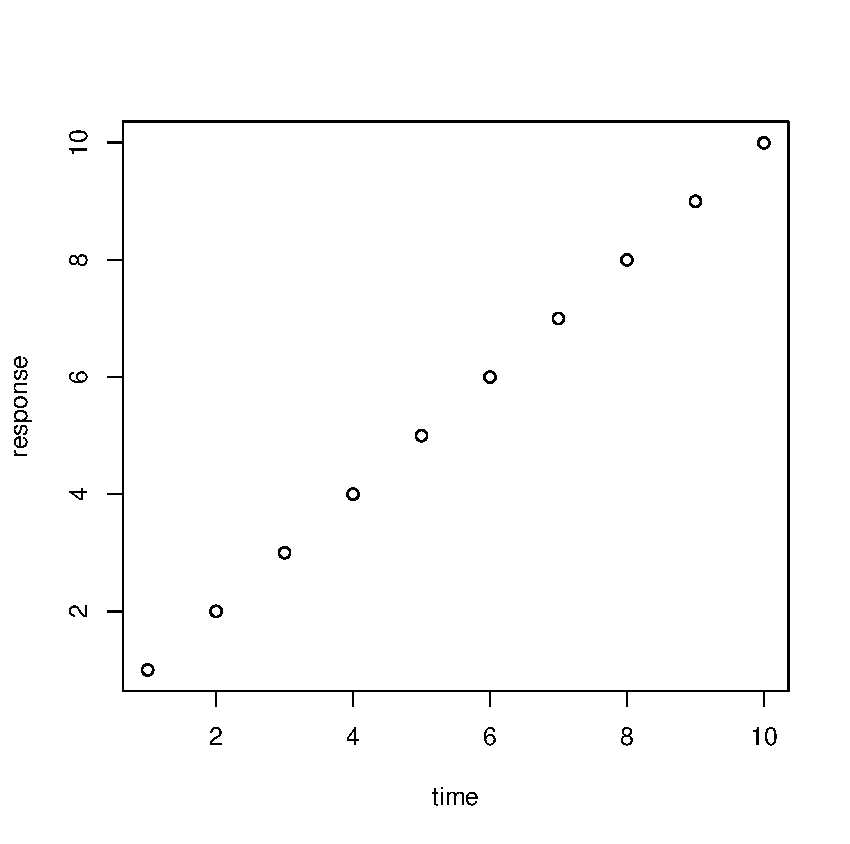
\includegraphics[width=3in,height=\textheight,keepaspectratio]{fig1.pdf}

}

\caption{\label{fig-first}Consistency comparison in fitting surrogate
model in the tidal power example.}

\end{figure}%

\subsection{Tables}\label{tables}

Making custom tables is easy. Do something like this:

\begin{longtable}[]{@{}lllll@{}}
\caption{Custom made tables}\label{tbl-one}\tabularnewline
\toprule\noalign{}
one & two & three & four & five \\
\midrule\noalign{}
\endfirsthead
\toprule\noalign{}
one & two & three & four & five \\
\midrule\noalign{}
\endhead
\bottomrule\noalign{}
\endlastfoot
1.23 & 3.45 & 5.00 & 1.21 & 3.41 \\
1.23 & 3.45 & 5.00 & 1.21 & 3.42 \\
1.23 & 3.45 & 5.00 & 1.21 & 3.43 \\
\end{longtable}

You can also input a table using raw latex syntax:

\begin{table}[!h] 
  \caption{Main results}\label{tbl-second} % Note that you need to use the latex syntax labeling here.
  \resizebox{\textwidth}{!}{
  \centering
\small % Reduce font size
\setlength{\tabcolsep}{4pt} % Adjust column spacing
\begin{tabular}{l *{7}{c}}
\toprule
& $(1)$ & $(2)$ & $(3)$ & $(4)$ & $(5)$ & $(6)$ & $(7)$ \\
\multicolumn{1}{c}{Dependent Variable} & All Waste & Trash & Food & Plastic & Textile & Metal & Can \\
\midrule
$\mathrm{WFH}$ & $-0.039$ & $0.061$ & $-0.110^{**}$ & $0.031^{**}$ & $0.010^{***}$ & $-0.006$ & $-0.010$\\
& $(0.128)$ & $(0.101)$ & $(0.051)$ & $(0.014)$ & $(0.004)$ & $(0.025)$ & $(0.011)$\vspace{1mm} \\
Adjusted $R^2$ & $0.481$ & $0.434$ & $0.475$ & $0.340$ & $0.141$ & $0.307$ & $0.256$\\
$\mathrm{N}$ & $972$ & $972$ & $972$ & $972$ & $972$ & $972$ & $972$\\
\bottomrule
\multicolumn{8}{p{.9\textwidth}}{\small \textbf{Notes.} Standard errors in parentheses are clustered at the district ($N=162$) level. $^{***}~\, \mathrm{p}<~0.01$; $^{**}\, \mathrm{p}< 0.05$ ; $^{*} \, \mathrm{p}<0.10$.}
\end{tabular}}
\end{table}

\begin{itemize}
\tightlist
\item
  Note that figures and tables (such as Figure~\ref{fig-first} and
  Table~\ref{tbl-one}, \ref{tbl-second}) should appear in the paper, not
  at the end or in separate files.
\end{itemize}

\begin{figure}

\centering{

\pandocbounded{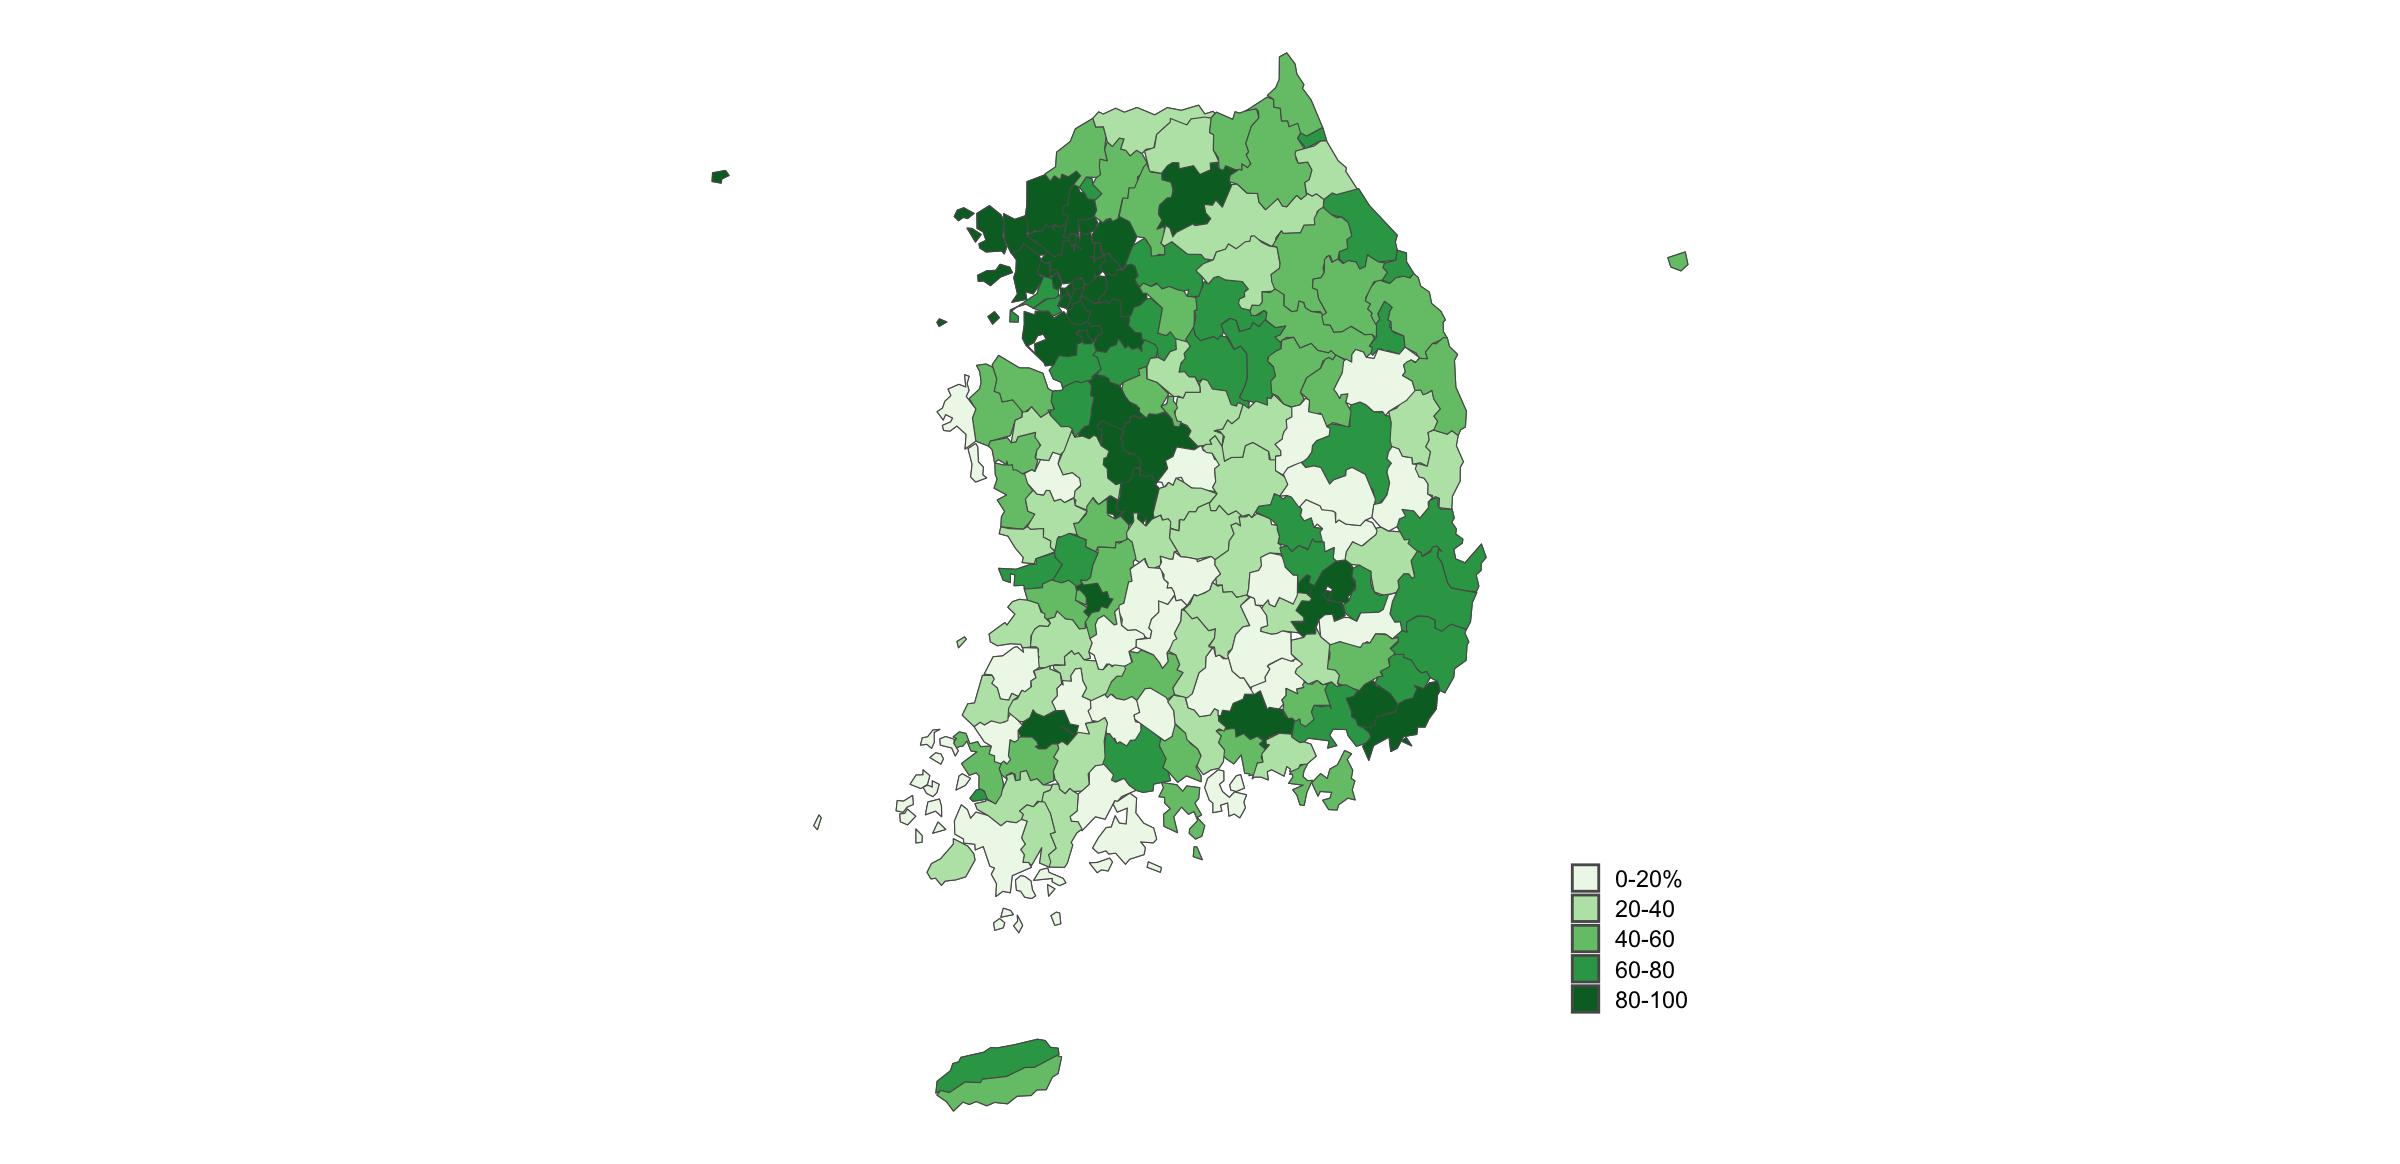
\includegraphics[keepaspectratio]{fig2.png}}

}

\caption{\label{fig-second}Map of Korea}

\end{figure}%

Another figure: Figure~\ref{fig-second}

\section{Related literature}\label{sec-lit}

Some citation example.

\citet{schott}: The famous international trade PNTR paper.

\citet{berlin}: Another famous paper in urban/spatial economics.

You can also put them inside the paranthesis: \citep{schott, berlin}.

Also, you can cite sections: Section~\ref{sec-lit}.

\section{Methods}\label{sec-meth}

Some few rounds of Lorem ipsums to give you a sense of the format:

Lorem ipsum. Lorem ipsum.Lorem ipsum.Lorem ipsum.Lorem ipsum.Lorem
ipsum.Lorem ipsum.Lorem ipsum.Lorem ipsum.Lorem ipsum.Lorem ipsum.Lorem
ipsum.Lorem ipsum.Lorem ipsum.Lorem ipsum.Lorem ipsum.Lorem ipsum.Lorem
ipsum.Lorem ipsum.Lorem ipsum.Lorem ipsum.Lorem ipsum.Lorem ipsum.Lorem
ipsum.Lorem ipsum.Lorem ipsum.Lorem ipsum.Lorem ipsum.Lorem ipsum.Lorem
ipsum.Lorem ipsum.Lorem ipsum.Lorem ipsum.Lorem ipsum.Lorem ipsum.Lorem
ipsum.Lorem ipsum.Lorem ipsum.Lorem ipsum.Lorem ipsum.Lorem ipsum.Lorem
ipsum.Lorem ipsum.Lorem ipsum.Lorem ipsum.Lorem ipsum.Lorem ipsum.Lorem
ipsum.Lorem ipsum.Lorem ipsum.Lorem ipsum.Lorem ipsum.Lorem ipsum.Lorem
ipsum.Lorem ipsum.Lorem ipsum.Lorem ipsum.Lorem ipsum.Lorem ipsum.Lorem
ipsum.Lorem ipsum.Lorem ipsum.Lorem ipsum.Lorem ipsum.Lorem ipsum.Lorem
ipsum.Lorem ipsum.Lorem ipsum.Lorem ipsum.Lorem ipsum.Lorem ipsum.Lorem
ipsum.Lorem ipsum.Lorem ipsum.Lorem ipsum.Lorem ipsum.Lorem ipsum.Lorem
ipsum.Lorem ipsum.Lorem ipsum.Lorem ipsum.

Lorem ipsum.Lorem ipsum.Lorem ipsum.Lorem ipsum.Lorem ipsum.Lorem
ipsum.Lorem ipsum.Lorem ipsum.Lorem ipsum.Lorem ipsum.Lorem ipsum.Lorem
ipsum.Lorem ipsum.Lorem ipsum.Lorem ipsum.Lorem ipsum.Lorem ipsum.Lorem
ipsum.Lorem ipsum.Lorem ipsum.Lorem ipsum.Lorem ipsum.Lorem ipsum.Lorem
ipsum.Lorem ipsum.Lorem ipsum.Lorem ipsum.Lorem ipsum.Lorem ipsum.Lorem
ipsum.Lorem ipsum.Lorem ipsum.Lorem ipsum.Lorem ipsum.Lorem ipsum.Lorem
ipsum.Lorem ipsum.Lorem ipsum.Lorem ipsum.Lorem ipsum.Lorem ipsum.Lorem
ipsum.Lorem ipsum.Lorem ipsum.Lorem ipsum.Lorem ipsum.Lorem ipsum.Lorem
ipsum.Lorem ipsum.Lorem ipsum.Lorem ipsum.Lorem ipsum.Lorem ipsum.Lorem
ipsum.Lorem ipsum.Lorem ipsum.Lorem ipsum.Lorem ipsum.Lorem ipsum.Lorem
ipsum.Lorem ipsum.Lorem ipsum.Lorem ipsum.Lorem ipsum.Lorem ipsum.Lorem
ipsum.Lorem ipsum.Lorem ipsum.Lorem ipsum.Lorem ipsum.Lorem ipsum.Lorem
ipsum.Lorem ipsum.Lorem ipsum.

Lorem ipsum.Lorem ipsum.Lorem ipsum.Lorem ipsum.Lorem ipsum.Lorem
ipsum.Lorem ipsum.Lorem ipsum.Lorem ipsum.Lorem ipsum.Lorem ipsum.Lorem
ipsum.Lorem ipsum.Lorem ipsum.Lorem ipsum.Lorem ipsum.Lorem ipsum.Lorem
ipsum.Lorem ipsum.Lorem ipsum.Lorem ipsum.Lorem ipsum.Lorem ipsum.Lorem
ipsum.Lorem ipsum.Lorem ipsum.Lorem ipsum.Lorem ipsum.Lorem ipsum.Lorem
ipsum.Lorem ipsum.Lorem ipsum.Lorem ipsum.Lorem ipsum.Lorem ipsum.Lorem
ipsum.Lorem ipsum.Lorem ipsum.Lorem ipsum.Lorem ipsum.Lorem ipsum.Lorem
ipsum.Lorem ipsum.Lorem ipsum.Lorem ipsum.Lorem ipsum.Lorem ipsum.Lorem
ipsum.Lorem ipsum.Lorem ipsum.Lorem ipsum.Lorem ipsum.Lorem ipsum.Lorem
ipsum.Lorem ipsum.Lorem ipsum.Lorem ipsum.Lorem ipsum.Lorem ipsum.Lorem
ipsum.Lorem ipsum.Lorem ipsum.Lorem ipsum.Lorem ipsum.Lorem ipsum.Lorem
ipsum.Lorem ipsum.Lorem ipsum.Lorem ipsum.Lorem ipsum.Lorem ipsum.Lorem
ipsum.Lorem ipsum.Lorem ipsum.Lorem ipsum.Lorem ipsum.Lorem ipsum.Lorem
ipsum.Lorem ipsum.Lorem ipsum.Lorem ipsum.

\section{Results}\label{sec-result}

I am not sure you would need this, but in quarto, you can directly type
codes and get their outputs (I know it's not pretty\ldots{} You can
customize it later if you want though):

\begin{Shaded}
\begin{Highlighting}[]
\FunctionTok{library}\NormalTok{(fixest)}

\NormalTok{mods }\OtherTok{=} \FunctionTok{feols}\NormalTok{(}
\NormalTok{  rating }\SpecialCharTok{\textasciitilde{}}\NormalTok{ complaints }\SpecialCharTok{+}\NormalTok{ privileges }\SpecialCharTok{+}\NormalTok{ learning }\SpecialCharTok{+} \FunctionTok{csw0}\NormalTok{(raises }\SpecialCharTok{+}\NormalTok{ critical),}
  \AttributeTok{data =}\NormalTok{ attitude}
\NormalTok{)}

\FunctionTok{summary}\NormalTok{(mods)}
\end{Highlighting}
\end{Shaded}

\begin{verbatim}
Standard-errors: IID 
Expl. vars.: complaints + privileges + learning
             Estimate Std. Error   t value   Pr(>|t|)    
(Intercept) 11.258305   7.318340  1.538369 1.3604e-01    
complaints   0.682416   0.128845  5.296434 1.5395e-05 ***
privileges  -0.103284   0.129345 -0.798515 4.3181e-01    
learning     0.237976   0.139410  1.707021 9.9735e-02 .  
---
Expl. vars.: complaints + privileges + learning + raises + critical
             Estimate Std. Error   t value   Pr(>|t|)    
(Intercept) 11.011130  11.703936  0.940806 0.35617817    
complaints   0.692053   0.148864  4.648883 0.00010141 ***
privileges  -0.103562   0.134730 -0.768665 0.44959057    
learning     0.249061   0.159619  1.560350 0.13176795    
raises      -0.033461   0.202276 -0.165420 0.86999856    
critical     0.015488   0.147250  0.105184 0.91710401    
\end{verbatim}

\section{Conclusion}\label{sec-conc}

\section*{References}\label{references}
\addcontentsline{toc}{section}{References}

\renewcommand{\bibsection}{}
\bibliography{bibliography.bib}

\phantomsection\label{appendix}
\bigskip

\begin{center}

{\large\bf APPENDIX}

\end{center}

\texttt{\{.supplementary\}} works as an indicator that makes the section
centered. Useful when starting an appendix or supplementary sections.

Section for Appendix.

\subsection*{Appendix A}\label{appendix-a}
\addcontentsline{toc}{subsection}{Appendix A}

Use \texttt{\{.unnumbered\}} to unnumber the section and give your own
numbering.

\subsection*{Appendix B}\label{appendix-b}
\addcontentsline{toc}{subsection}{Appendix B}

\phantomsection\label{supplementary}
\bigskip

\begin{center}

{\large\bf SUPPLEMENTARY}

\end{center}





\end{document}
